%% LyX 2.2.0 created this file.  For more info, see http://www.lyx.org/.
%% Do not edit unless you really know what you are doing.
\documentclass[spanish,oneside,mathserif,notheorems]{beamer}
\usepackage[latin9]{inputenc}
\setcounter{secnumdepth}{3}
\setcounter{tocdepth}{3}
\usepackage{graphicx}

\makeatletter
%%%%%%%%%%%%%%%%%%%%%%%%%%%%%% Textclass specific LaTeX commands.
 % this default might be overridden by plain title style
 \newcommand\makebeamertitle{\frame{\maketitle}}%
 % (ERT) argument for the TOC
 \AtBeginDocument{%
   \let\origtableofcontents=\tableofcontents
   \def\tableofcontents{\@ifnextchar[{\origtableofcontents}{\gobbletableofcontents}}
   \def\gobbletableofcontents#1{\origtableofcontents}
 }

%%%%%%%%%%%%%%%%%%%%%%%%%%%%%% User specified LaTeX commands.
\usetheme[pageofpages=de,% String used between the current page and thetotal page count.
          bullet=circle,% Use circles instead of squares for bullets.
          titleline=true,% Show a line below the frame title.
          alternativetitlepage=true,% Use the fancy title page.
          titlepagelogo=../graphics/logo.png,% Logo for the first page.
          ]{Torino}
% Nouvelle is a green and red alternative to the chameleon color theme.
\usecolortheme{freewilly}
%\usecolortheme{nouvelle}

\newcommand{\monthname}{\ifcase\month\or Enero\or Febrero\or
      Marzo\or Abril\or Mayo\or Junio\or Julio\or Agosto\or Septiembre\or
      Octubre\or Noviembre\or Diciembre\fi}

%Usando para definicion
\usepackage{amsthm}
\setbeamertemplate{theorems}[numbered]
\theoremstyle{definition} 
\newtheorem{definition}{Definici�n}[section]

\makeatother

\usepackage{babel}
\addto\shorthandsspanish{\spanishdeactivate{~<>}}

\begin{document}

\title{Reconocimiento de Actividades Humanas con un enfoque colaborativo}

\subtitle{Tesis de Grado}

\author{Alberto Gimenez\\
Santiago Yegros}

\institute{Facultad Polit�cnica}

\date{\monthname, \the\year}
\makebeamertitle
\begin{frame}

\frametitle<presentation>{Contenido}

\tableofcontents[hideothersubsections]{} 
\end{frame}
%
\AtBeginSection[]
{
	\begin{frame}
		\frametitle{Contenido}        		\tableofcontents[currentsection]
%\tableofcontents[currentsection, currentsubsection,  hideothersubsections,    subsectionstyle=show/shaded,  ] 
	\end{frame} 
}


\section{Introducci�n}

\subsection{Definici�n del Problema}
\begin{frame}{Definici�n del Problema}

\framesubtitle{Reconocimiento de Actividades Humanas}
\begin{overprint}
\onslide<1> 
\begin{quote}
Determinar las acciones o comportamientos de uno o m�s individuos
a partir de datos ambiguos capturados por sensores situados en el
entorno.
\end{quote}
\onslide<2> 
\begin{block}<2>{Nota}
\emph{}El problema es conocido por sus siglas \structure{HAR} en
ingl�s \emph{(Human Activity Recognition})
\end{block}
\end{overprint}
\begin{center}
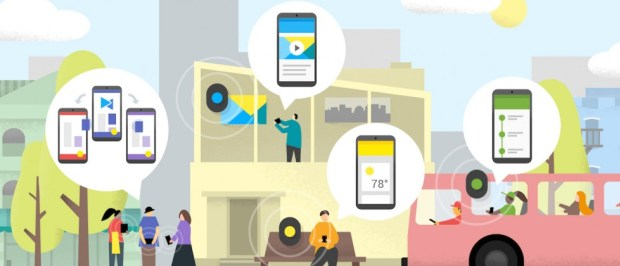
\includegraphics[width=0.8\textwidth]{intro/graphics/sensor-environment}
\par\end{center}

\end{frame}
%
\begin{frame}{Definici�n del Problema}

\setbeamercovered{transparent}

\framesubtitle{�Que es HAR?}
\begin{itemize}[<+->]
\item Es un t�pico de investigaci�n multidisciplinario que busca dise�ar
algoritmos para:
\begin{itemize}
\item Capturar movimientos de uno o m�s individuos en interacci�n con su
entorno 
\item Realizar aprendizaje e inferencia
\item Proveer informaci�n de contexto 
\end{itemize}
\end{itemize}
\begin{overprint}
\onslide<2> 
\begin{center}
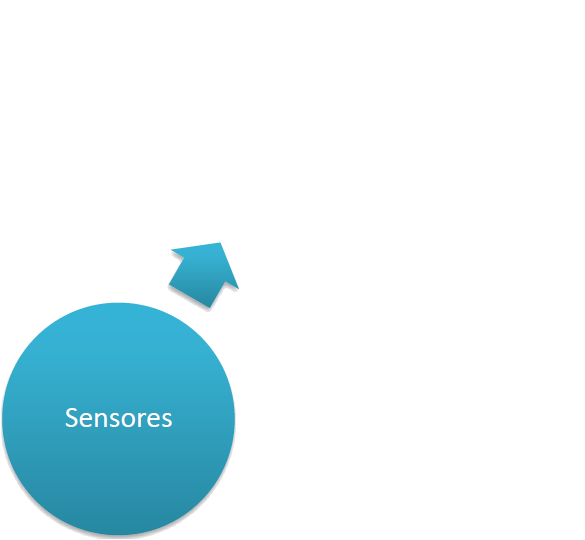
\includegraphics[width=4.5cm]{intro/graphics/areas-1}
\par\end{center}
\onslide<3> 
\begin{center}
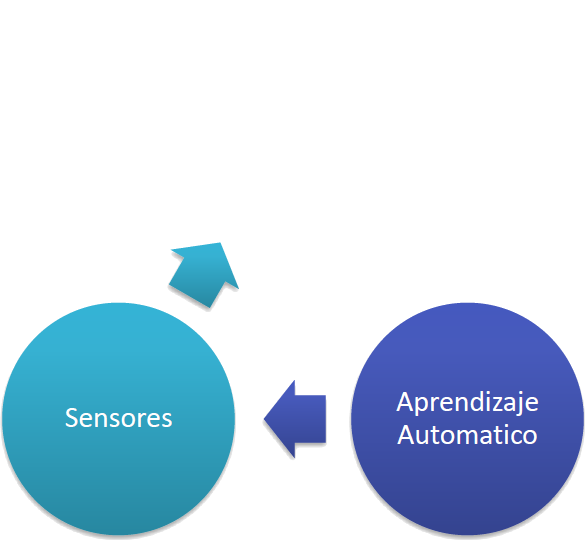
\includegraphics[width=4.5cm]{intro/graphics/areas-2}
\par\end{center}
\onslide<4> 
\begin{center}
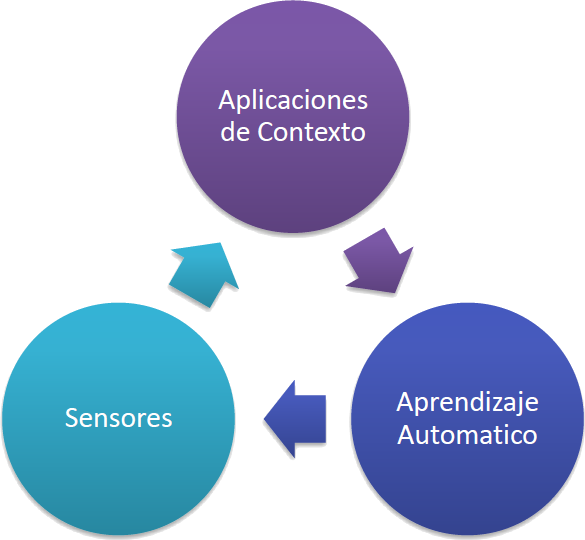
\includegraphics[width=4.5cm]{intro/graphics/areas-3}
\par\end{center}

\end{overprint}
\end{frame}
%
\begin{frame}{Definici�n del Problema}

\framesubtitle{Motivaci�n\setlength\columnsep{0pt}}
\begin{columns}

\column{0.5\textwidth}
\begin{itemize}[<+->]
\item El \structure{contexto} es primordial para los sistemas inteligentes 
\item Avances en tecnolog�as de \structure{computaci�n m�vil} y \structure{sensores} 
\item Uso intensivo de \structure{tel�fonos m�viles modernos} en la vida
diaria.
\item \setbeamercovered{transparent}Popularidad de \structure{aplicaciones m�viles}
de contexto en 
\begin{itemize}
\item el cuidado personal, 
\item la movilidad y 
\item la asistencia en la vida diaria 
\end{itemize}
\end{itemize}

\column{0.5\textwidth}
\begin{overprint}
\onslide<1> 
\begin{center}

\includegraphics[width=1\textwidth]{intro/graphics/context1}
\par\end{center}
\onslide<2> 
\begin{center}
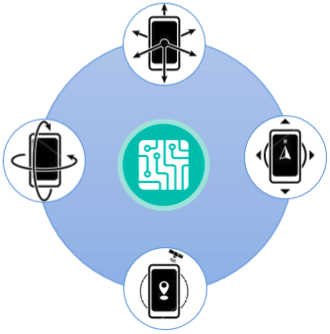
\includegraphics[width=1\textwidth]{intro/graphics/sensors}
\par\end{center}
\onslide<3> 

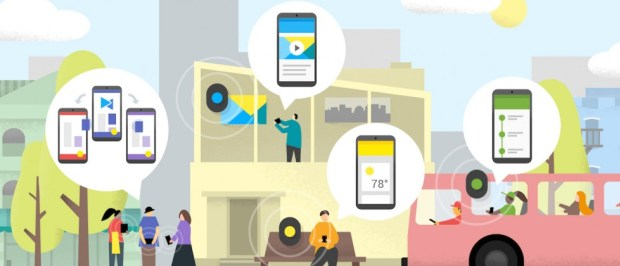
\includegraphics[bb=100bp 0bp 520bp 266bp,clip,width=1\textwidth]{intro/graphics/sensor-environment}
\onslide<4-> 


\includegraphics[width=1\textwidth]{intro/graphics/mobile-phone}

\end{overprint}
\end{columns}

\end{frame}
%
\begin{frame}[shrink]{Definici�n del Problema}

\framesubtitle{Actividades Humanas}

\setbeamercovered{transparent}
\begin{block}{Actividades Simples}
Acciones simples peri�dicas de larga duraci�n.
\end{block}
\begin{center}
\uncover<2->{\begin{center}
\begin{tabular}{|c|>{\raggedright}p{5cm}|}
\hline 
Ambulatorias & Caminar, correr, sentarse, pararse, quieto, acostarse, subir y descender
escaleras.\tabularnewline
\hline 
Transporte & En bus, bicicleta y conducir.\tabularnewline
\hline 
\end{tabular}
\par\end{center}}
\par\end{center}
\begin{block}{Actividades Complejas}
Acciones cortas o peri�dicas no comunes.
\end{block}
\begin{center}
\uncover<3->{\begin{center}
\begin{tabular}{|c|>{\raggedright}p{5cm}|}
\hline 
Cotidianas & Comer, beber, mirar TV, leer, cepillarse los dientes, entre otros.\tabularnewline
\hline 
Gimnasio & Alzar pesas, ejercicio aer�bico, bicicleta est�tica.\tabularnewline
\hline 
Militares & Arrastrarse, en cuclillas.\tabularnewline
\hline 
\end{tabular}
\par\end{center}}
\par\end{center}

\end{frame}
%




\subsection{Alcance}
\begin{frame}{Alcance}

\framesubtitle{Propuesta}
\begin{center}
Reconocer actividades humanas utilizando tel�fonos m�viles modernos
con un enfoque colaborativo
\par\end{center}

\end{frame}
%
\begin{frame}{Alcance}

\framesubtitle{Objetivo General}
\begin{center}
El objetivo principal es desarrollar un sistema \structure{HAR} utilizando
tel�fonos m�viles modernos cuyo aporte principal es un una librer�a
de c�digo abierto y un modelo activo.
\par\end{center}

\end{frame}
%
\begin{frame}{Alcance}

\framesubtitle{Objetivos Espec�ficos}

\setbeamercovered{transparent}
\begin{enumerate}[<+->]
\item Definir el marco te�rico sobre \structure{HAR}. 
\item Revisar las t�cnicas de \structure{captura de se�ales} bajo restricci�n
de consumo de energ�a. 
\item Revisar el \structure{procesamiento de se�ales} para identificar
variables de entrenamiento. 
\item Comprender la clasificaci�n basada \structure{aprendizaje autom�tico}
bajo restricci�n de consumo energ�a. 
\item Dise�ar un \structure{sistema HAR} que incluya la recolecci�n de
muestras colaborativas y clasificaci�n de actividades en-l�nea. 
\item Aportar un componente de \structure{librer�a} para tel�fonos m�viles
modernos con plataforma \emph{\textbf{\emph{Android}}}. 
\end{enumerate}
\end{frame}
%
\begin{frame}{Alcance}

\framesubtitle{Actividades Humanas}

\setbeamercovered{transparent}
\begin{columns}[t]

\column{0.25\textwidth}
\begin{itemize}
\item Acciones cortas

\pause{}
\item Actividades Simples

\pause{}
\item Actividades Complejas
\begin{itemize}
\item Combinaci�n
\item Cotidianas 
\item Gimn�sticas
\item Militares
\end{itemize}

\pause{}
\end{itemize}

\column{0.75\textwidth}
\begin{overprint}
\onslide<1-3> 
\begin{center}
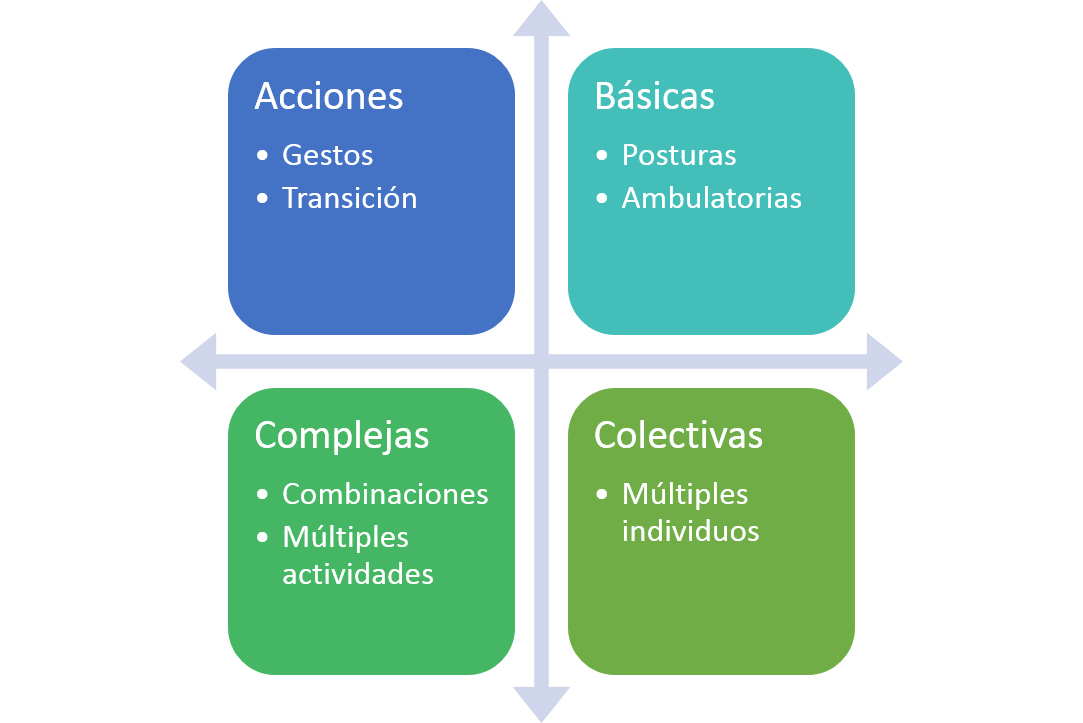
\includegraphics[width=0.95\columnwidth]{propuesta/graphics/actividades}
\par\end{center}
\onslide<4> 
\begin{center}
\begin{tabular}{|l|>{\raggedright}p{4cm}|}
\hline 
\textbf{Grupo}  & \textbf{Ejemplos} \tabularnewline
\hline 
\hline 
Posturas & Sentarse, Pararse, Estar quieto\tabularnewline
\hline 
Ambulatorias  & Caminar, correr, subir o descender escaleras.\tabularnewline
\hline 
Transporte  & Andar en bus, en bicicleta o en veh�culo\tabularnewline
\hline 
Cotidianas & Comer, beber, mirar TV, leer, cepillarse los dientes, entre otros. \tabularnewline
\hline 
Ejercitarse  & Alzar pesas, bicicleta est�tica y aer�bicos. \tabularnewline
\hline 
\end{tabular}
\par\end{center}
\end{overprint}
\end{columns}

\end{frame}




\section{Metodolog�a HAR}

\begin{frame}[t]{Metodolog�a HAR}
\framesubtitle{Definici�n Te�rica}

\begin{block}{Problema HAR} 

Dado un conjunto $W=\{w_{0},...,w_{m-1}\}$ con $m$ ventanas de tiempo \\~\ 

donde cada $w_{j}$ contiene series de tiempo $S_{j}=\{s_{j,0},...,s_{j,k-1}\}$ para $k$ se�ales \\~\ \par

Y un conjunto $A\text{=}\{\mathrm{a}_{0},...,\mathrm{a}_{n-1}\}$ de actividades \\~\

El objetivo es encontrar $\mathbf{  F\colon S_{j}\rightarrow A }$ para todos los $S_{j}$ en cada $w_{j}$ \\~\
\end{block}

\end{frame}
%
\begin{frame}{Metodolog�a HAR}
\framesubtitle{Proceso de aprendizaje}
	\begin{center}
		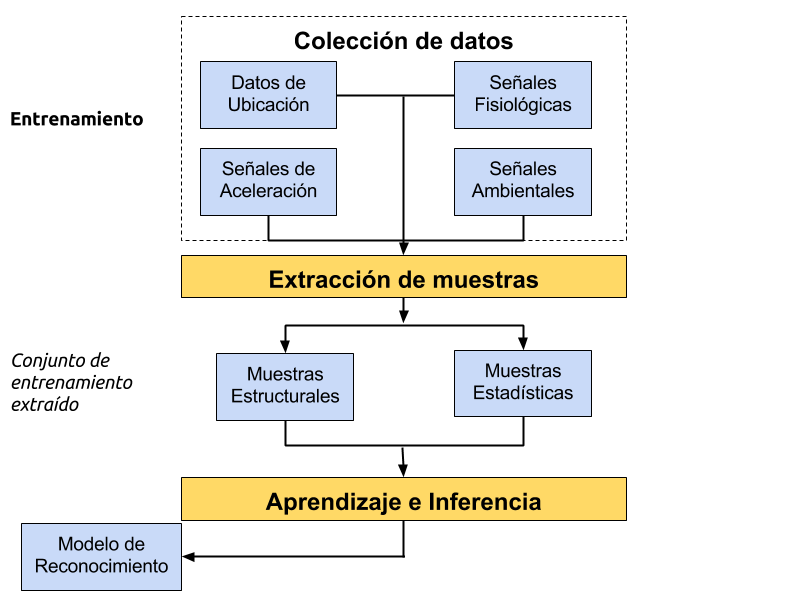
\includegraphics[width=8cm]{propuesta/graphics/har-3}
		\par
	\end{center}
\end{frame}
%
\begin{frame}{Metodolog�a HAR}
\framesubtitle{Proceso de evaluaci�n}
	\begin{center}
		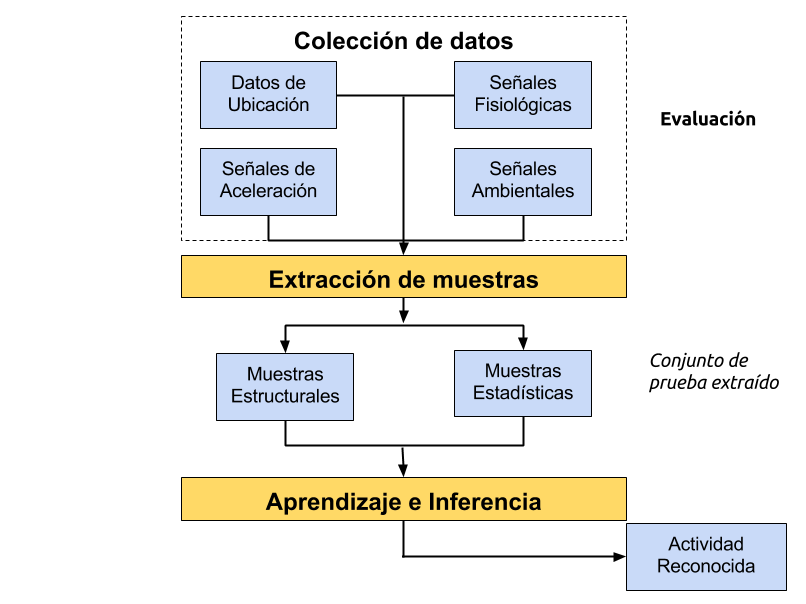
\includegraphics[width=8cm]{propuesta/graphics/har-6}
		\par
	\end{center}
\end{frame}
%
\begin{frame}{Metodolog�a HAR}
\framesubtitle{Proceso HAR}
	\begin{center}
		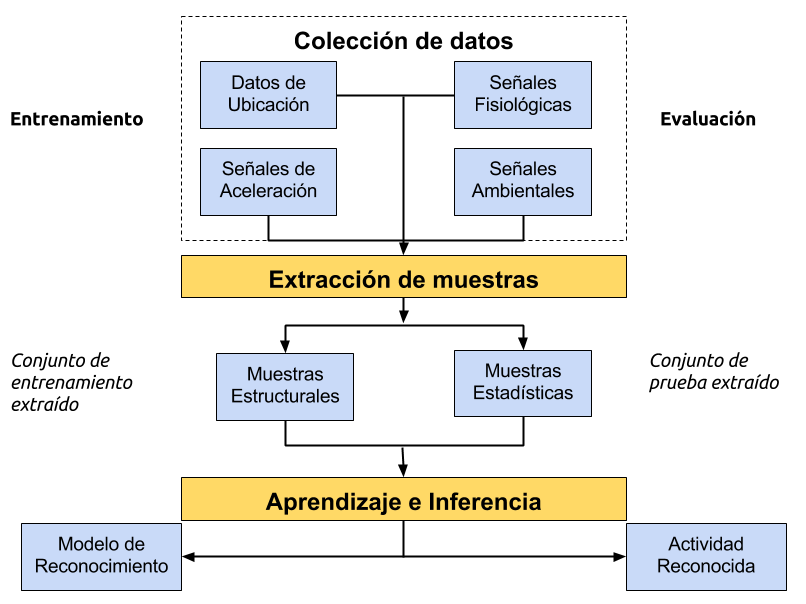
\includegraphics[width=8cm]{propuesta/graphics/har-7}
		\par
	\end{center}
\end{frame}
%
\begin{frame}{Metodolog�a HAR}
\framesubtitle{Colecci�n de Datos}
El primer paso es recolectar se�ales obtenidas de sensores unidos al cuerpo (cintura, mu�eca, muslos, etc) realizando alguna actividad de inter�s.

\begin{center}
\resizebox{\linewidth}{!}{
\begin{tabular}{|c|c|c|c|c|c|c|c|}
	\hline 
	\multicolumn{8}{|c|}{Sensores} \\ 
	\hline 
	\multicolumn{2}{|c|}{Movimiento}	& \multicolumn{2}{c|}{Posici�n} 	& \multicolumn{2}{c|}{Ambientales}  	& \multicolumn{2}{c|}{Fisiol�gicas}  		\\ 
	\hline 
	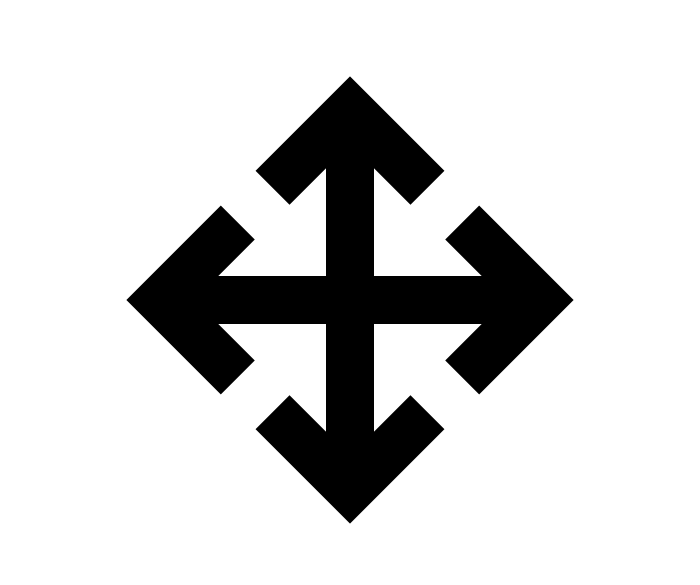
\includegraphics[width=0.05\textwidth]{propuesta/graphics/acelerometro} 	& Acelerometro 		&
	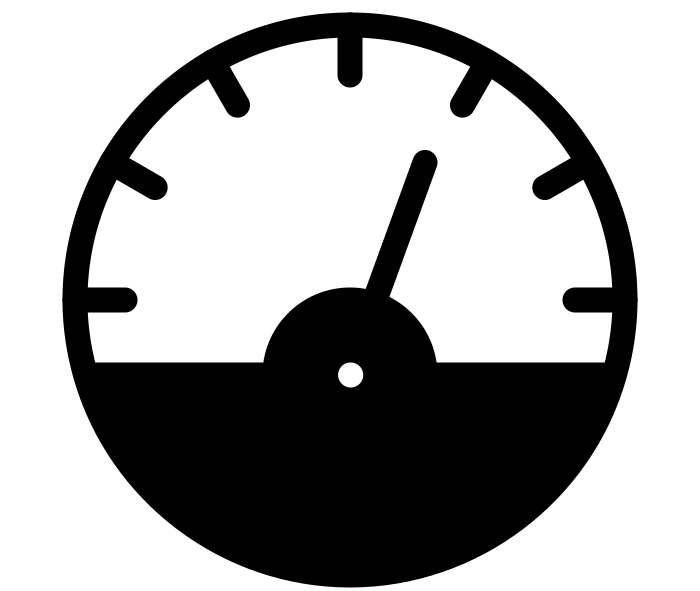
\includegraphics[width=0.04\textwidth]{propuesta/graphics/barometro}		& Bar�metro			&
	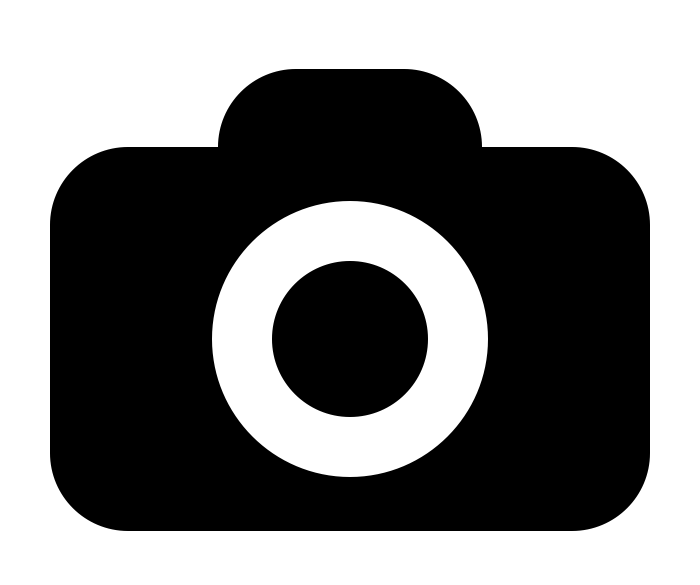
\includegraphics[width=0.05\textwidth]{propuesta/graphics/camera}			& Camara			&
	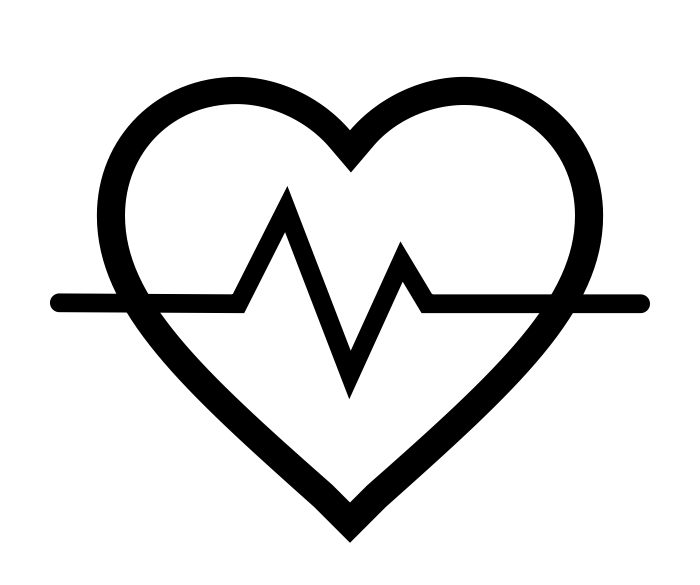
\includegraphics[width=0.05\textwidth]{propuesta/graphics/ritmo_cardiaco}	& Ritmo Card�aco	
	\\
	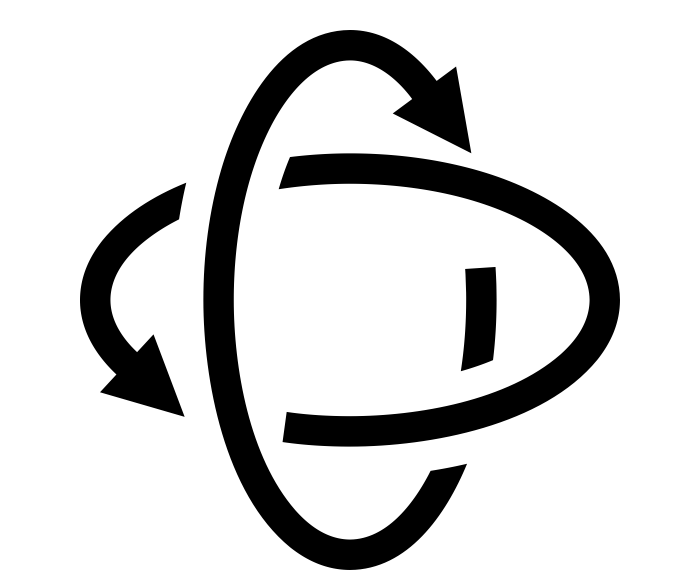
\includegraphics[width=0.05\textwidth]{propuesta/graphics/giroscopio} 		& Giroscopio 		&
	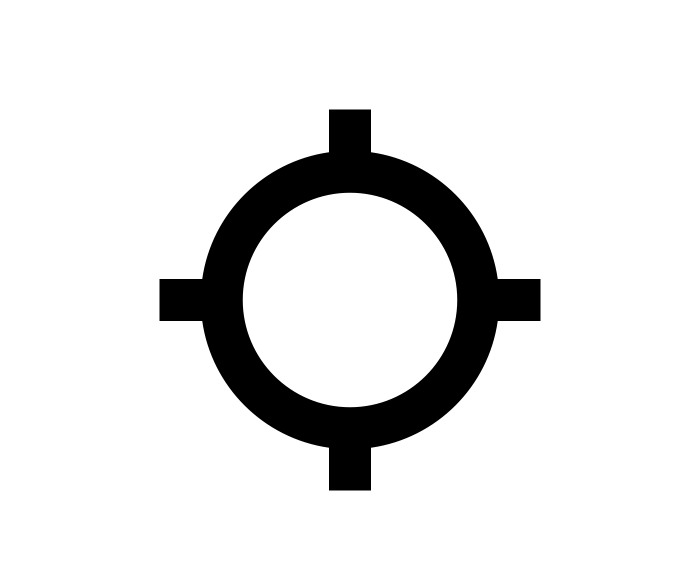
\includegraphics[width=0.05\textwidth]{propuesta/graphics/gps}				& GPS				&
	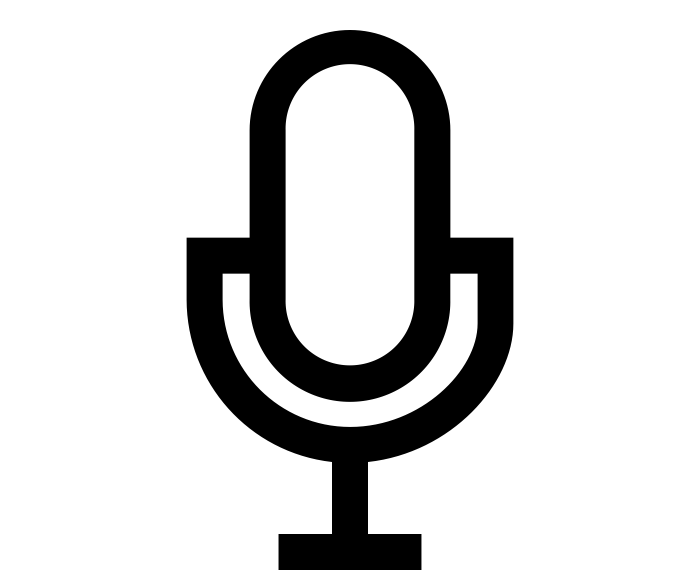
\includegraphics[width=0.05\textwidth]{propuesta/graphics/microfono}		& Micr�fono			&
	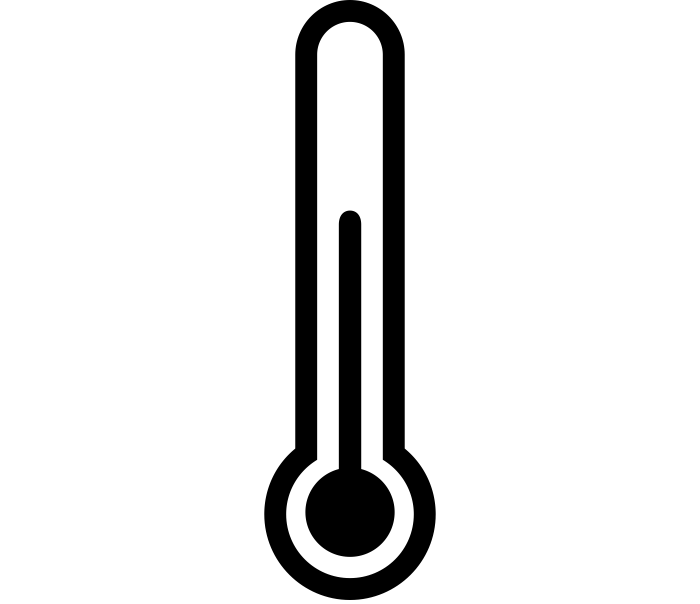
\includegraphics[width=0.05\textwidth]{propuesta/graphics/temperatura}		& Temperatura		
	\\
	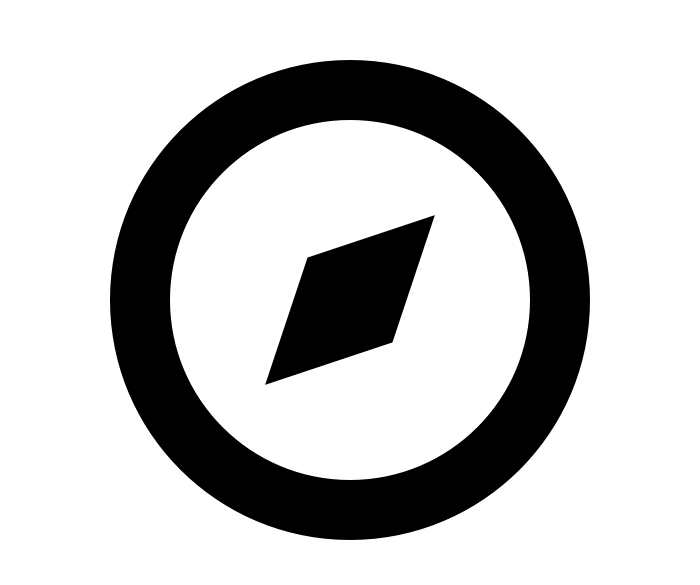
\includegraphics[width=0.05\textwidth]{propuesta/graphics/magnetometro} 	& Magnet�metro		&
	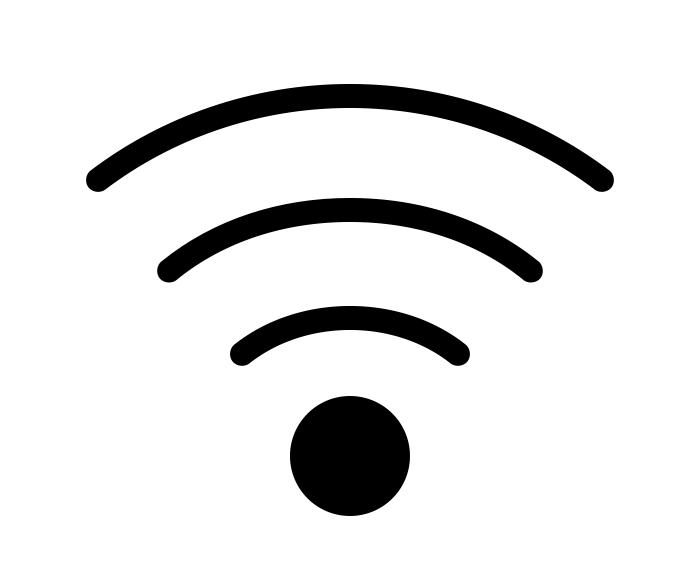
\includegraphics[width=0.05\textwidth]{propuesta/graphics/wifi}				& WIFI				&
	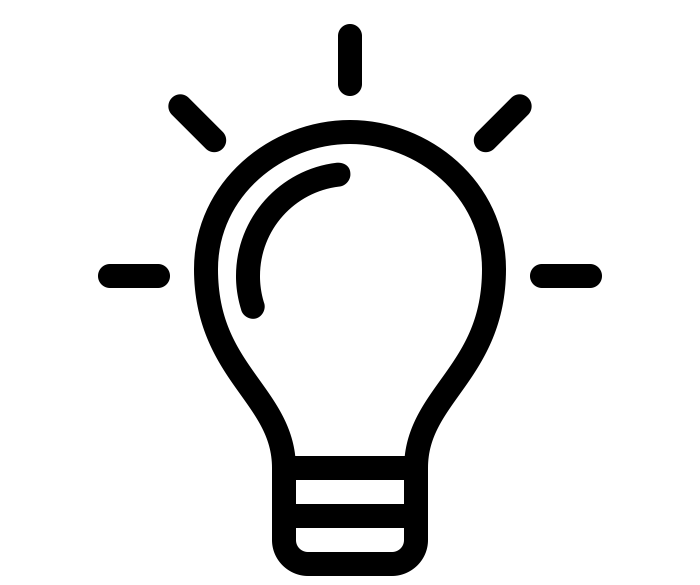
\includegraphics[width=0.05\textwidth]{propuesta/graphics/luz}				& Luz				&
																				&  						
	\\
	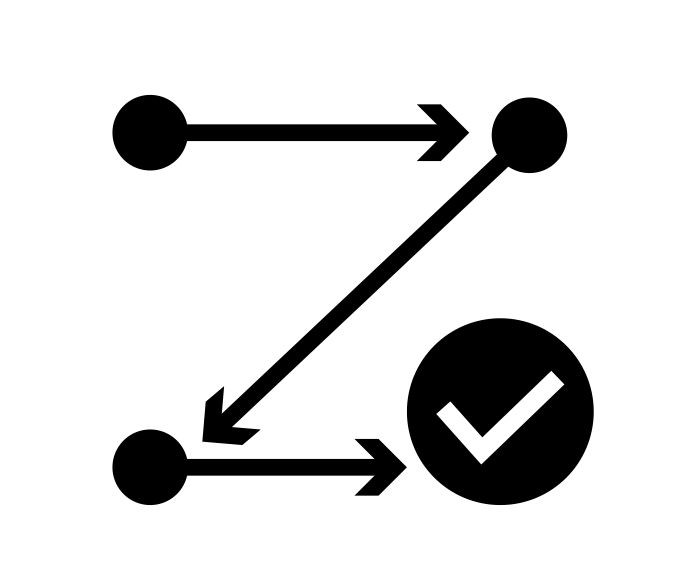
\includegraphics[width=0.05\textwidth]{propuesta/graphics/pedometro}		& Pod�metro			&	
	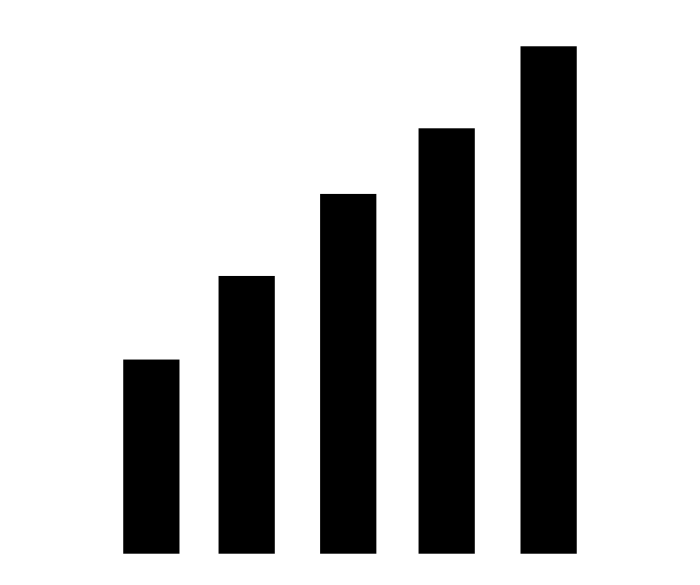
\includegraphics[width=0.05\textwidth]{propuesta/graphics/gsm}				& GSM				&
	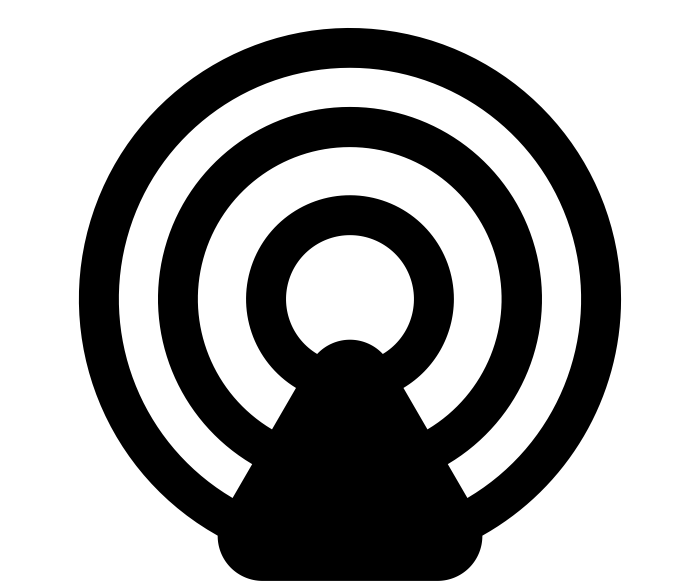
\includegraphics[width=0.05\textwidth]{propuesta/graphics/proximidad}		& Proximidad		&	
																				&					
	\\
	\hline 
\end{tabular}
} % fin del resize
\end{center}
\end{frame}
%
\begin{frame}{Metodolog�a HAR}
\framesubtitle{Extracci�n de Muestras}
	\begin{itemize}
		\setlength\itemsep{1em}
		\item El siguiente paso es el procesamiento de las se�ales obtenidas por los sensores y extraer las caracter�sticas relevantes de los datos sin procesar.
		\item El procesamiento de muestra se basa en cuatro tareas distintas:
		\begin{itemize}
			\item Etiquetado.
			\item Suavizado.
			\item Muestreo.
			\item Extracci�n de Caracter�sticas.
		\end{itemize}
	\end{itemize}
\end{frame}
%
\begin{frame}{Metodolog�a HAR}
\framesubtitle{Extracci�n de Muestras}
\begin{columns}
	
\column{4cm}
	\begin{itemize}[<+->]
		\setlength\itemsep{1em}
		\item \underline{Etiquetado}: Los datos de los sensores se deben recopilar y etiquetar.
		\item \underline{Suavizado}: Los sensores electr�nicos pueden introducir cierta inestabilidad en la se�al (jitter) para reducir esto se aplica uno o mas filtros. 
	\end{itemize}


\column{6cm}
	\begin{overprint}
		\onslide<1> 
		\begin{center}
			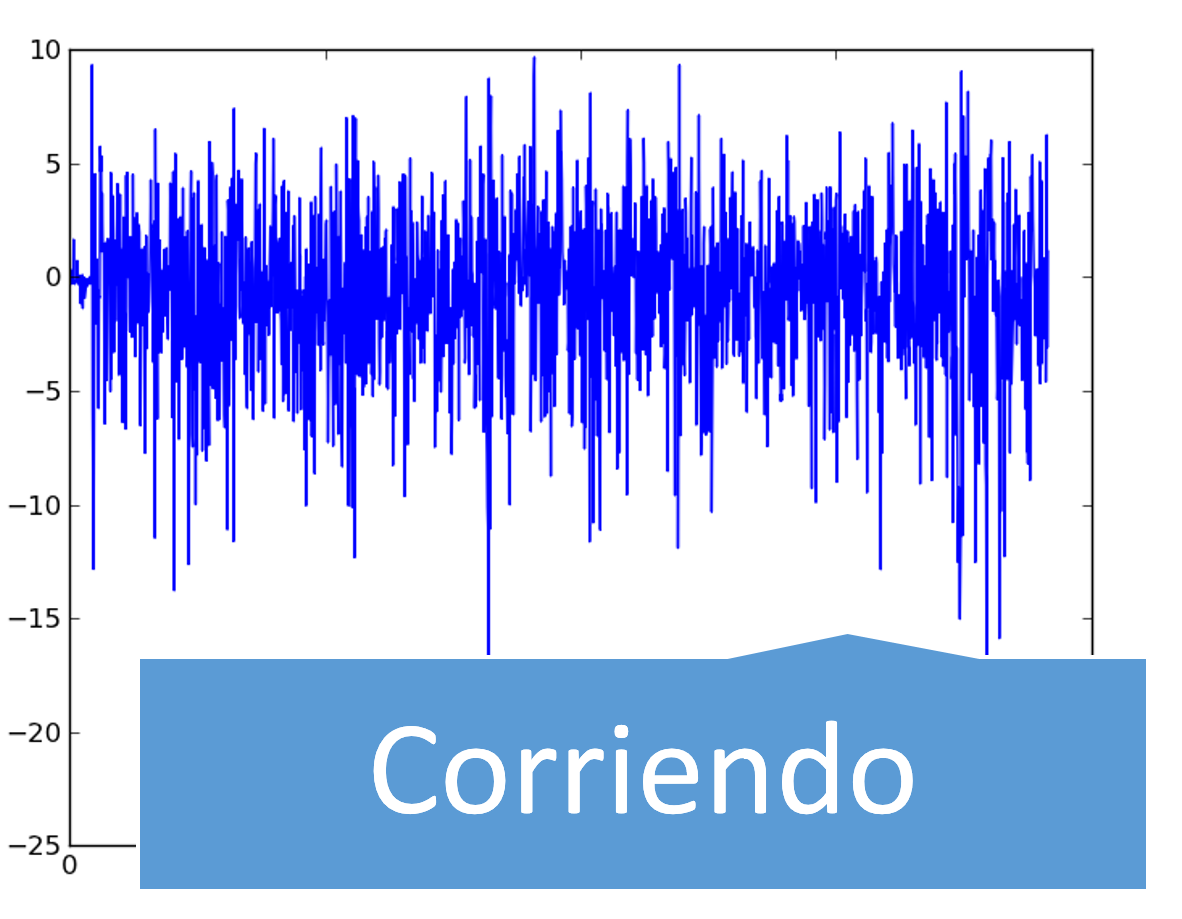
\includegraphics[width=\textwidth]{propuesta/graphics/labelled}
			\par
		\end{center}
		\onslide<2> 
		\begin{center}
			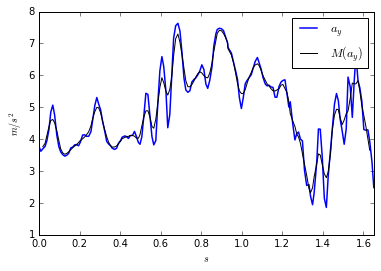
\includegraphics[width=\textwidth]{propuesta/graphics/moving_average}
			\par
		\end{center}
		
	\end{overprint}
\end{columns}
\end{frame}
%
\begin{frame}{Metodolog�a HAR}
\framesubtitle{Extracci�n de Muestras - Muestreo}
\begin{columns}
	
\column{5.2cm}
	\begin{itemize}[<+->]
		\setlength\itemsep{1em}
		\item \underline{Muestreo}: Los datos colectados se segmentan en ventanas de tiempo discretas.
		\item \underline{Extracci�n de Caracter�sticas}: El proceso de extracci�n consiste en extraer valores caracter�sticos en cada ventana de tiempo.
	\end{itemize}

\column{4.8cm}
	\begin{overprint}
	\onslide<1> 
	\begin{center}
		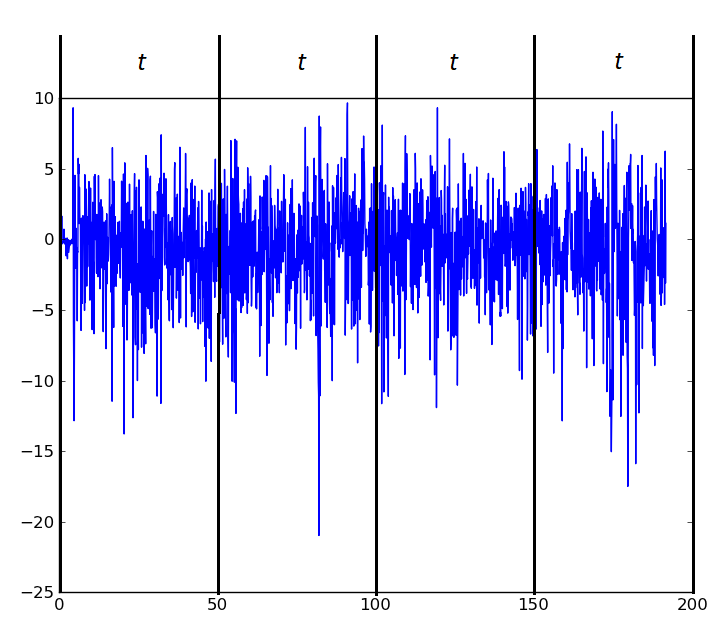
\includegraphics[width=5.2cm]{propuesta/graphics/muestreo}
		\par
	\end{center}
	\onslide<2> 
	\begin{center}
		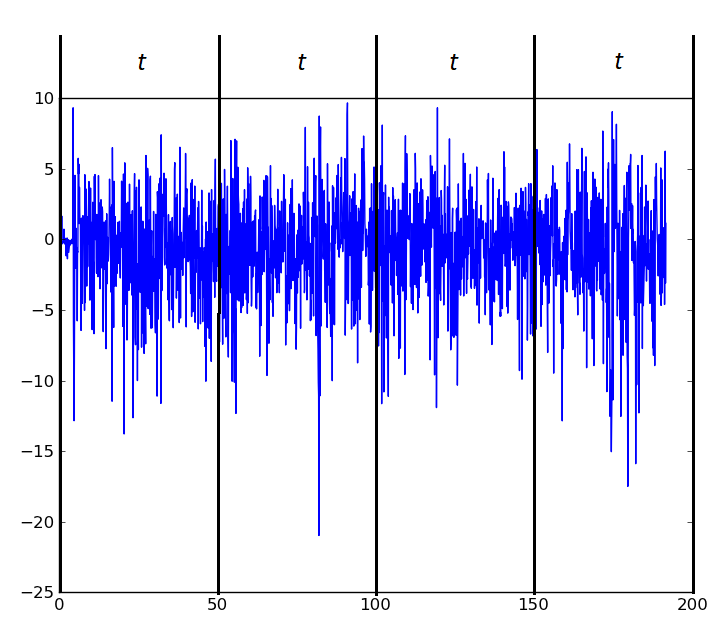
\includegraphics[width=5.2cm]{propuesta/graphics/muestreo}
		\par
	\end{center}
	\end{overprint}

\end{columns}
\end{frame}
%
\begin{frame}{Metodolog�a HAR}	
\framesubtitle{Extracci�n de Muestras}
Las m�tricas estad�sticas con respecto al tiempo y frecuencia:
\par
\begin{table}
\centering
\resizebox{8cm}{!}{
	\begin{tabular}{|l|l|}
		\hline 
		Funci�n & M�trica \tabularnewline
		\hline 
		\hline 
		\texttt{mean(s)} 			& Media Aritm�tica			\tabularnewline
		\hline 
		\texttt{std(s)} 			& Desviaci�n est�ndar \tabularnewline
		\hline 
		\texttt{max(s)} 			& Valor m�ximo \tabularnewline
		\hline 
		\texttt{min(s)} 			& Valor m�nimo \tabularnewline
		\hline 
		\texttt{skewness(s)} 		& Asimetr�a \tabularnewline
		\hline 
		\texttt{kurtosis(s)} 		& Kurtosis \tabularnewline
		\hline 
		\texttt{energy(s)} 			& Energ�a \tabularnewline
		\hline 
		\texttt{entropy(s)} 		& Entrop�a \tabularnewline
		\hline 
		\texttt{irq(s)} 			& Rango intercuartil \tabularnewline
		\hline 
		\texttt{autoregression(s)} 	& Coeficientes autorregresivos \tabularnewline
		\hline 
		\texttt{meanFreq(s)} 		& Promedio en frecuencia \tabularnewline
		\hline 
	\end{tabular}
	\par
}
\end{table}
\end{frame}
%
\begin{frame}{Metodolog�a HAR}	
\framesubtitle{Aprendizaje e inferencia}
\begin{itemize}
	\setlength\itemsep{1em}
	\item Un HAR es similar a cualquier aplicaci�n de aprendizaje autom�tico. 
	\item El objetivo principal del algoritmo es clasificar los datos desconocidos.
	\item Hay muchos algoritmos de clasificaci�n: 
	\begin{itemize}
		\item Arboles de Decisi�n
		\item SVM
		\item Clasificadores de Bayes, 
		\item Modelos de Markov
		\item Redes Neuronales y otros.
	\end{itemize}
\end{itemize}
\end{frame}
%
\begin{frame}
{Metodolog�a HAR}	
\framesubtitle{�rbol de Decisi�n}
\begin{columns}
	
\column{0.57\textwidth}
	\begin{itemize}[<+->]
		\item M�todo de aprendizaje predictivo sobre un conjunto de instancias etiquetadas.
		\item Cada nodo interno denota una prueba de un atributo, y cada nodo hoja es una etiqueta o clase.
		\item Utiliza el criterio de proporci�n de ganancia.
		\item Simple de Implementar.
		\item Algoritmos de J. R. Quinlan ID3, C4.5 (Implementaci�n Java j48 de WEKA).
	\end{itemize}
	
	
\column{0.43\textwidth}
	\begin{overprint}
		\onslide<1-5> 
		\begin{center}
			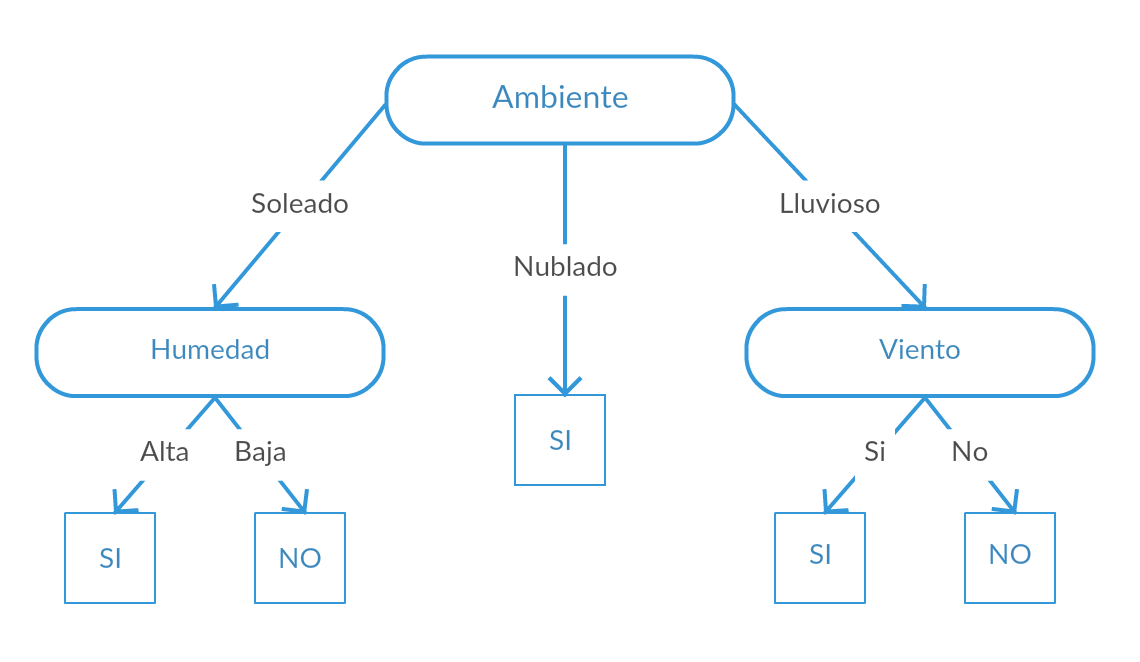
\includegraphics[width=\textwidth]{propuesta/graphics/dtree}
			\par
		\end{center}

	\end{overprint}
\end{columns}
\end{frame}
%
\begin{frame}[fragile]{Metodolog�a HAR}
\framesubtitle{�rbol de Decisi�n - Algoritmo}

\begin{center}
	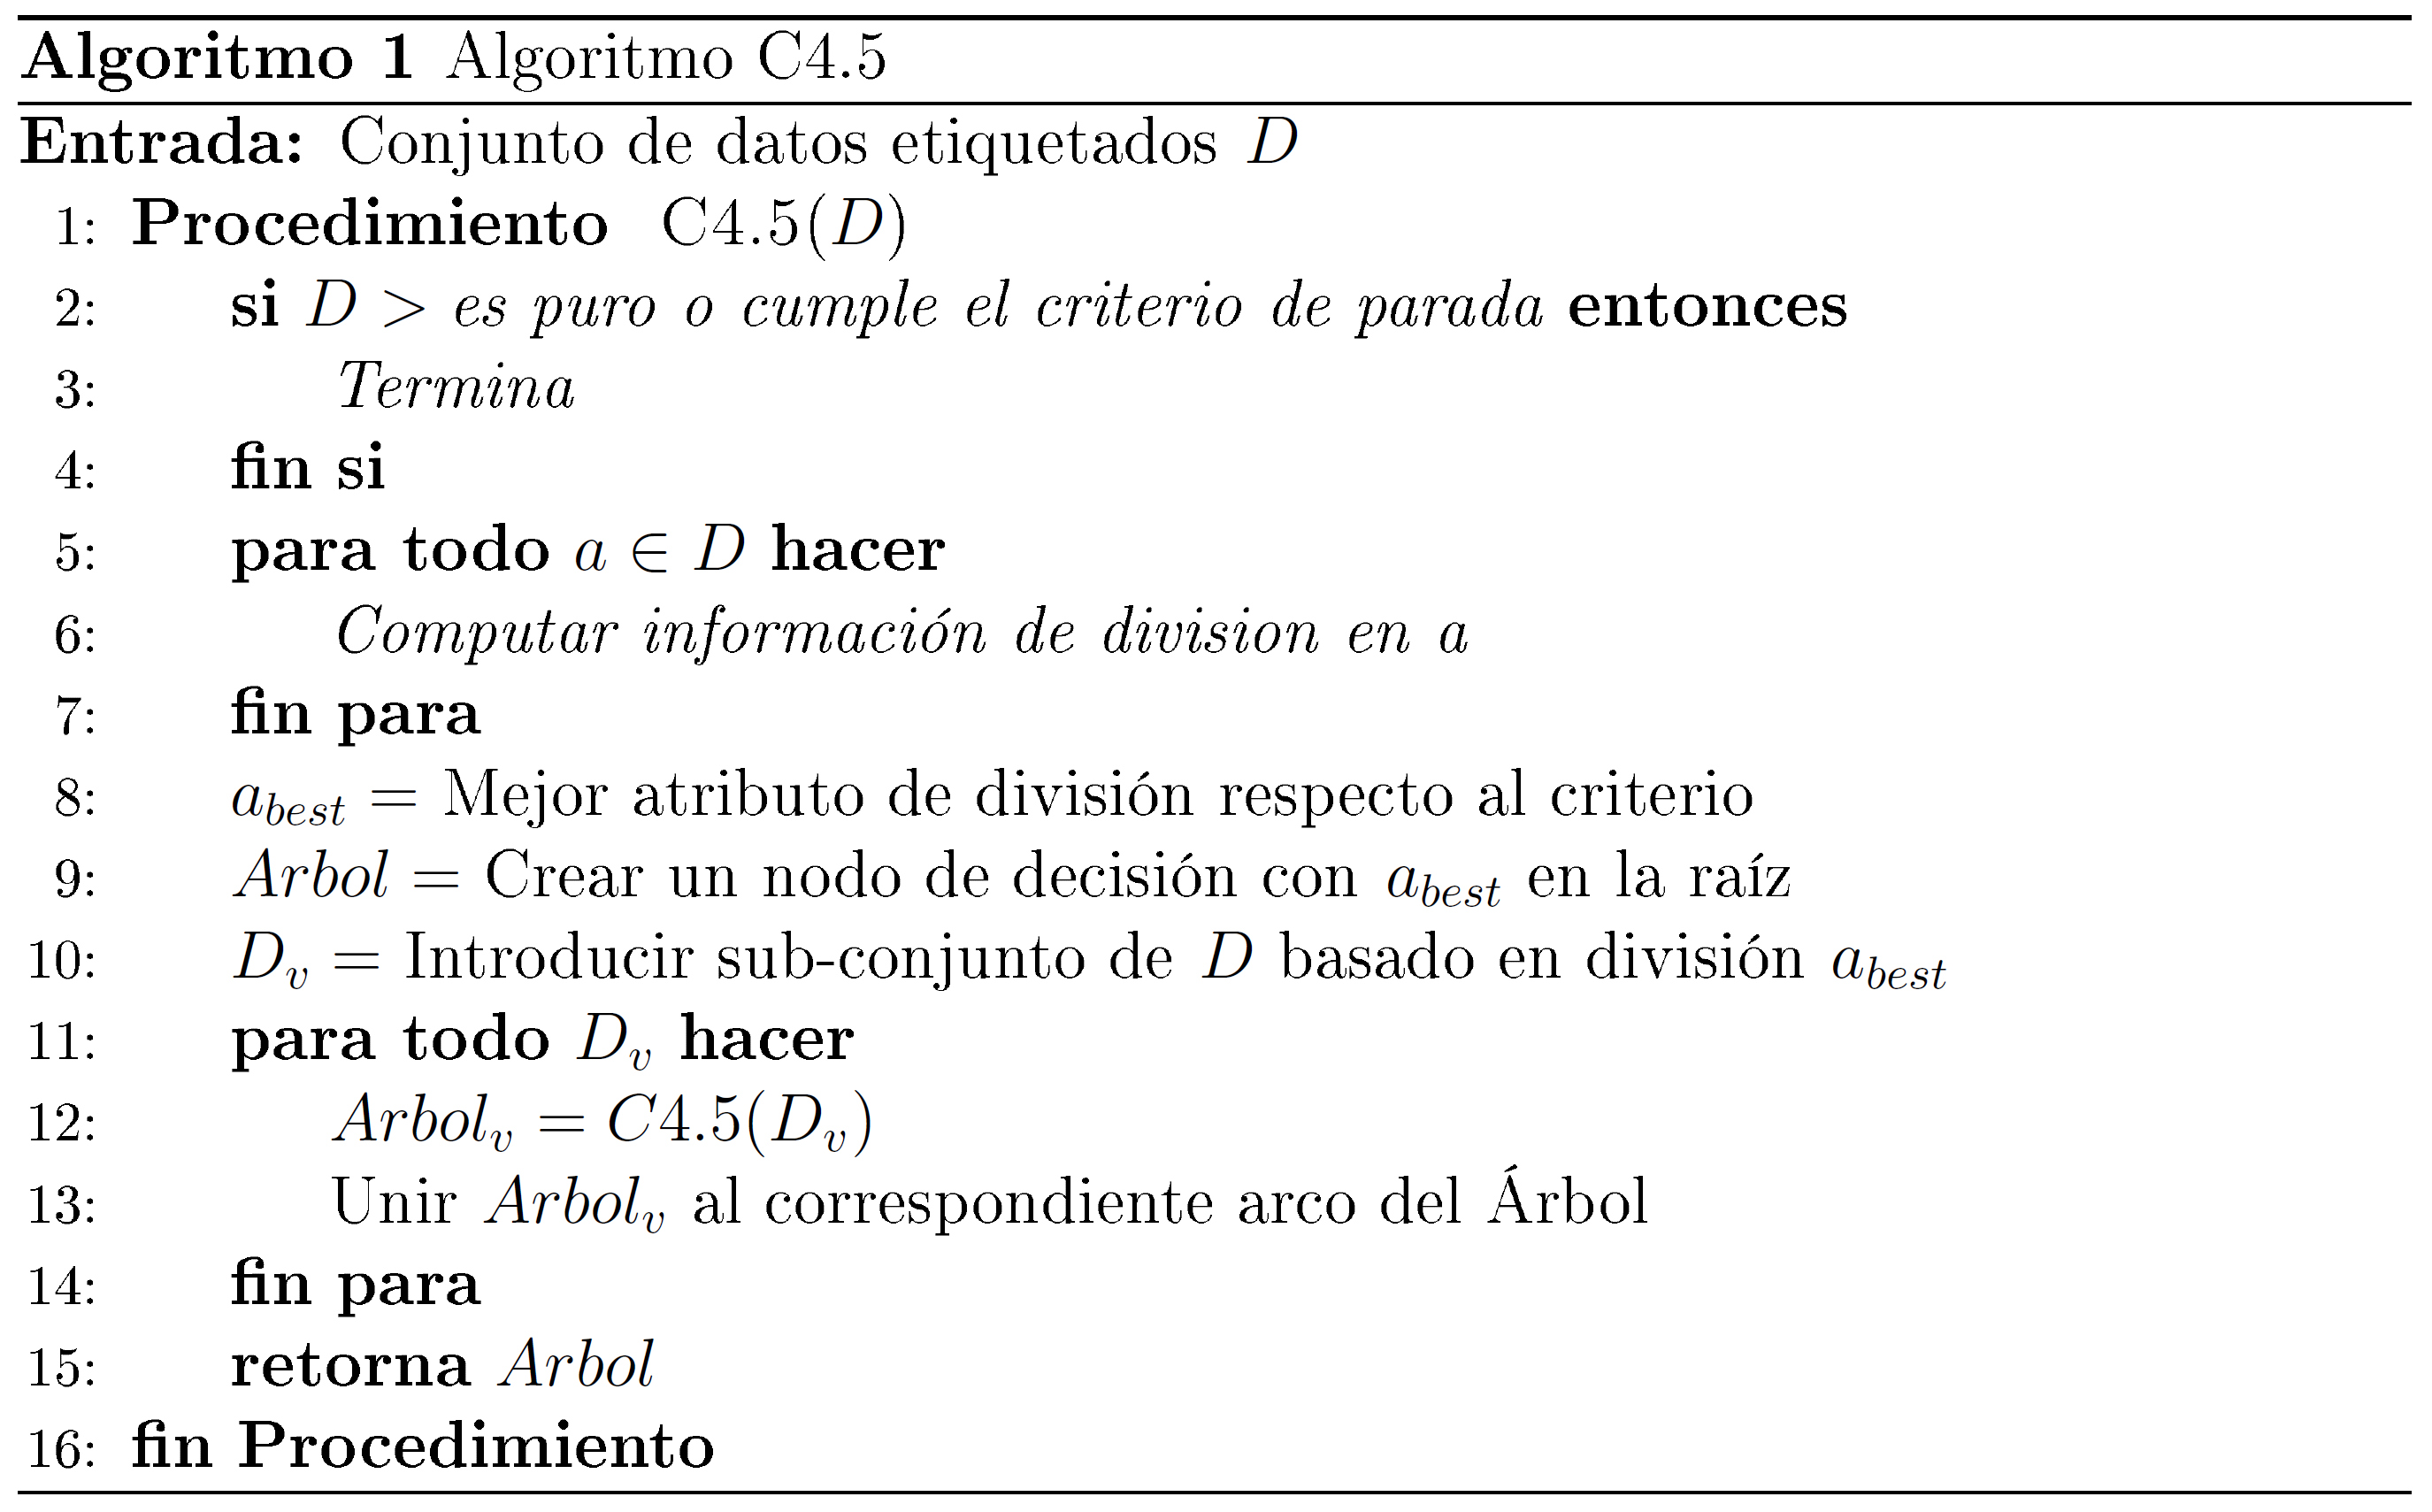
\includegraphics[width=\textheight]{propuesta/graphics/algoritmoC45}
	\par
\end{center}

\end{frame}



\section{Sistemas HAR}
\begin{frame}{Sistemas HAR}

\framesubtitle{Aplicaciones de Contexto}

\setbeamercovered{transparent}
\begin{itemize}
\item Aplicaciones cuyo medio de interacci�n incluye al contexto.
\end{itemize}

\pause{}
\begin{itemize}
\item El contexto es el estado acerca de la informaci�n
\begin{itemize}
\item f�sica,
\item emocional,
\item social, entre otros
\end{itemize}
\end{itemize}

\pause{}
\begin{itemize}
\item La computaci�n m�vil y ubicua es sin�nimo de dinamismo en el contexto
\end{itemize}

\pause{}
\begin{itemize}
\item Los tipos de contexto comunes en la computaci�n m�vil son: 
\begin{itemize}
\item la ubicaci�n, 
\item la identidad, 
\item la actividad 
\item y el tiempo
\end{itemize}
\end{itemize}
\end{frame}
%
\begin{frame}<article>{Sistemas HAR}

\framesubtitle{Prop�sito del sistema}

\setbeamercovered{transparent}
\begin{itemize}
\item Proveer un componente para el desarrollo de aplicaciones de contexto. 
\end{itemize}

\pause{}
\begin{itemize}
\item Reconocer actividades realizadas rutinariamente de diferentes maneras, 
\begin{itemize}
\item por diferentes usuarios y 
\item en diferentes contextos.
\end{itemize}

\pause{}
\item Reconocer actividades mediante el uso de sensores.
\end{itemize}

\pause{}
\begin{itemize}
\item Ser portado oportunamente como atuendo para los usuarios (\emph{Wearable})
\end{itemize}
\end{frame}
%
\begin{frame}{Sistemas HAR}

\framesubtitle{Dise�o del sistema}

\setbeamercovered{transparent}
\begin{itemize}
\item Arquitectura basada en aplicaciones de aprendizaje autom�tico.
\end{itemize}

\pause{}
\begin{itemize}
\item Componentes principales
\begin{itemize}
\item un \structure{recolector} de medidas 
\item un \structure{procesador} de muestras 
\item un \structure{clasificador} de actividades
\end{itemize}
\end{itemize}

\pause{}
\begin{itemize}
\item Metodolog�a operativa
\begin{itemize}
\item Aprendizaje fuera de linea (\emph{off-line})
\item Clasificaci�n en linea (\emph{on-line})
\end{itemize}
\end{itemize}
\begin{center}
\visible<2->{\begin{center}
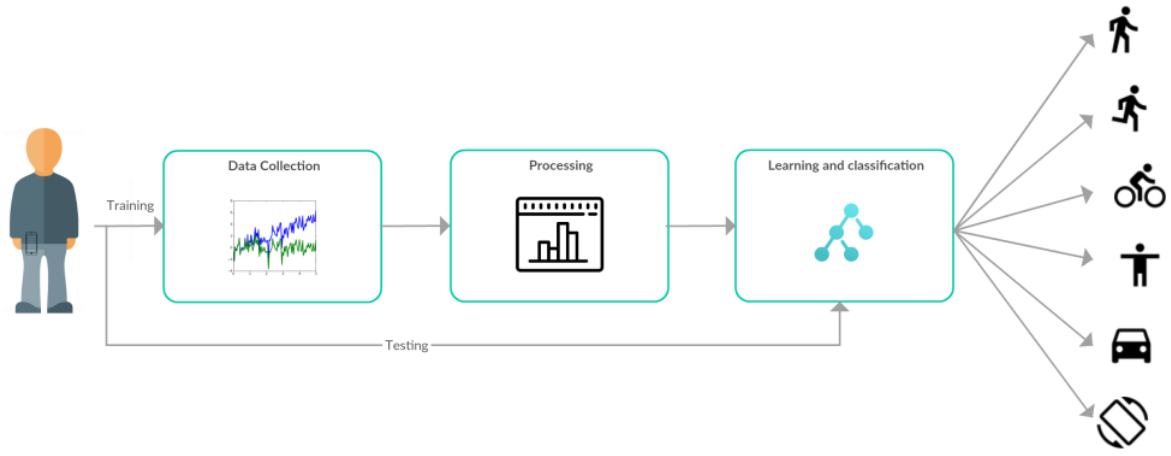
\includegraphics[width=0.6\textwidth]{../capitulo-2/graphics/harsystem2}
\par\end{center}}
\par\end{center}

\end{frame}
%
\begin{frame}{Sistemas HAR}

\framesubtitle{Componentes del sistema}

\setbeamercovered{transparent}
\begin{columns}

\column{0.25\textwidth}
\begin{itemize}
\item Recolector
\begin{itemize}
\item Sensor
\item Registro
\end{itemize}
\end{itemize}

\pause{}
\begin{itemize}
\item Procesador
\begin{itemize}
\item Filtro
\item Extracci�n
\end{itemize}
\end{itemize}

\pause{}
\begin{itemize}
\item Clasificador
\begin{itemize}
\item Aprendizaje
\item Clasificaci�n
\end{itemize}
\end{itemize}

\column{0.75\textwidth}

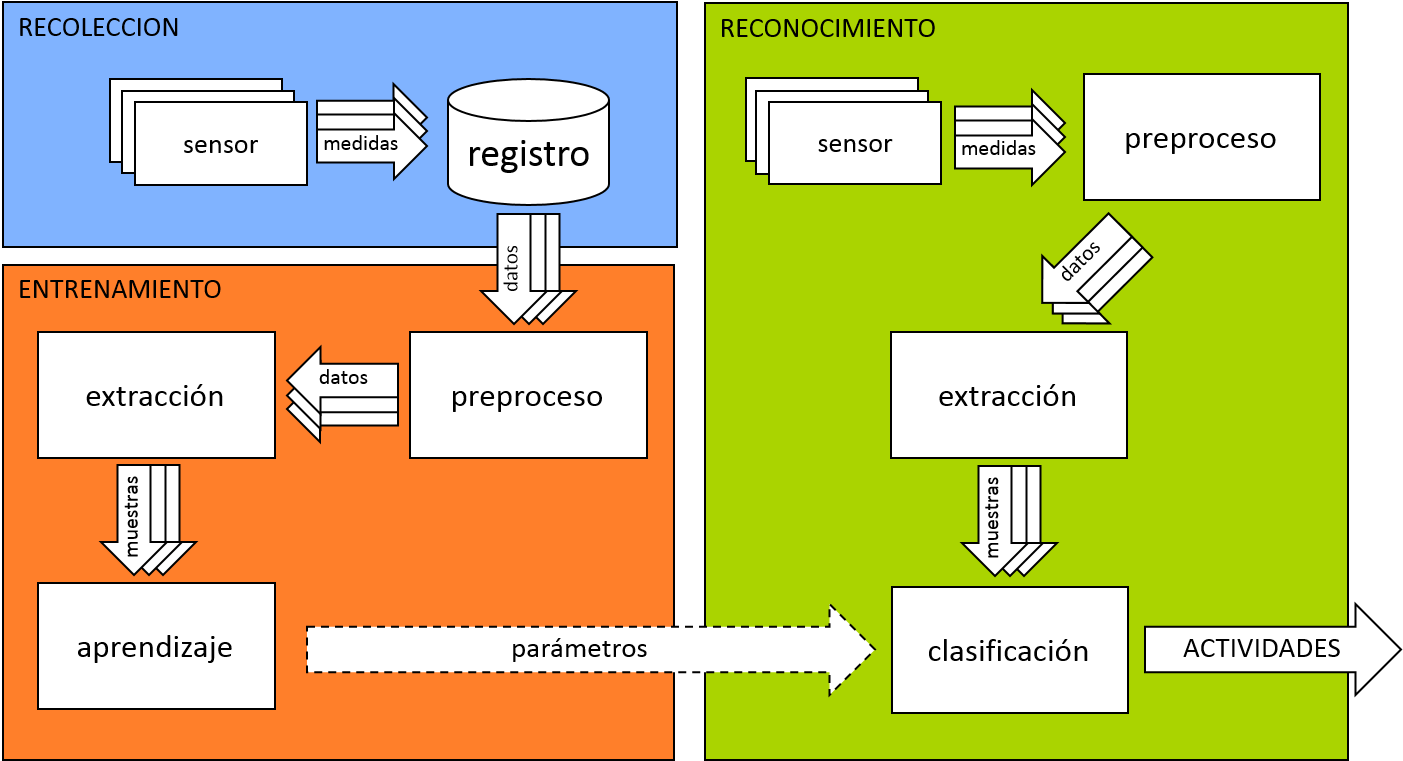
\includegraphics[width=1\columnwidth]{propuesta/graphics/harsystem}
\end{columns}

\end{frame}




\section{HAR en Android}
\begin{frame}{HAR en Android}

\framesubtitle{Arquitectura del Proyecto}

\setbeamercovered{transparent}
\begin{columns}

\column{0.5\textwidth}
\begin{itemize}
\item \textbf{HARDroid} 
\begin{itemize}
\item Es un servicio utilitario de reconocimiento.
\item Clasificador din�mico (\structure{DEX})
\end{itemize}

\pause{}
\item \textbf{ActivitySurvey}
\begin{itemize}
\item Aplicaci�n de encuesta que depende del servicio.
\item Registra evaluaciones de los usuarios. 
\end{itemize}

\pause{}
\item \textbf{Backend C4.5} 
\begin{itemize}
\item Servicio web de recolecci�n de evaluaciones.
\item Los aciertos son utilizados para mejorar el clasificador.
\end{itemize}
\end{itemize}

\column{0.5\textwidth}
\begin{center}
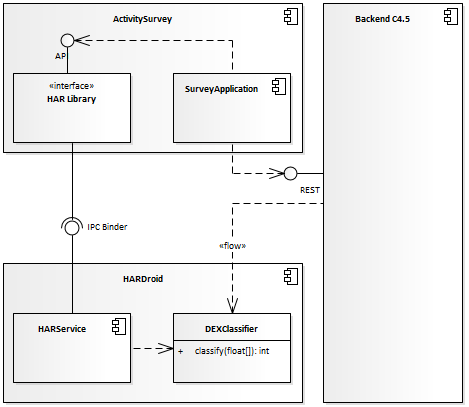
\includegraphics[width=1\columnwidth]{../capitulo-5/graphics/arqui_general}
\par\end{center}

\end{columns}

\end{frame}
%
\begin{frame}{HAR en Android}

\framesubtitle{Servicio de Reconocimiento}

\setbeamercovered{transparent}
\begin{columns}

\column{0.5\textwidth}
\begin{itemize}[<+->]
\item \structure{HARDroid} es un gestor en la capa de \emph{Application Framework}. 
\item Modelo \structure{Cliente-Servidor}.
\item Las aplicaciones m�viles hechas por terceros obtienen: 
\begin{itemize}
\item mejoras del motor de reconocimiento, 
\item actualizaci�n por plataforma de distribuci�n basado en tienda, 
\item mecanismos f�ciles de integraci�n.
\end{itemize}
\end{itemize}

\column{0.5\textwidth}
\begin{center}
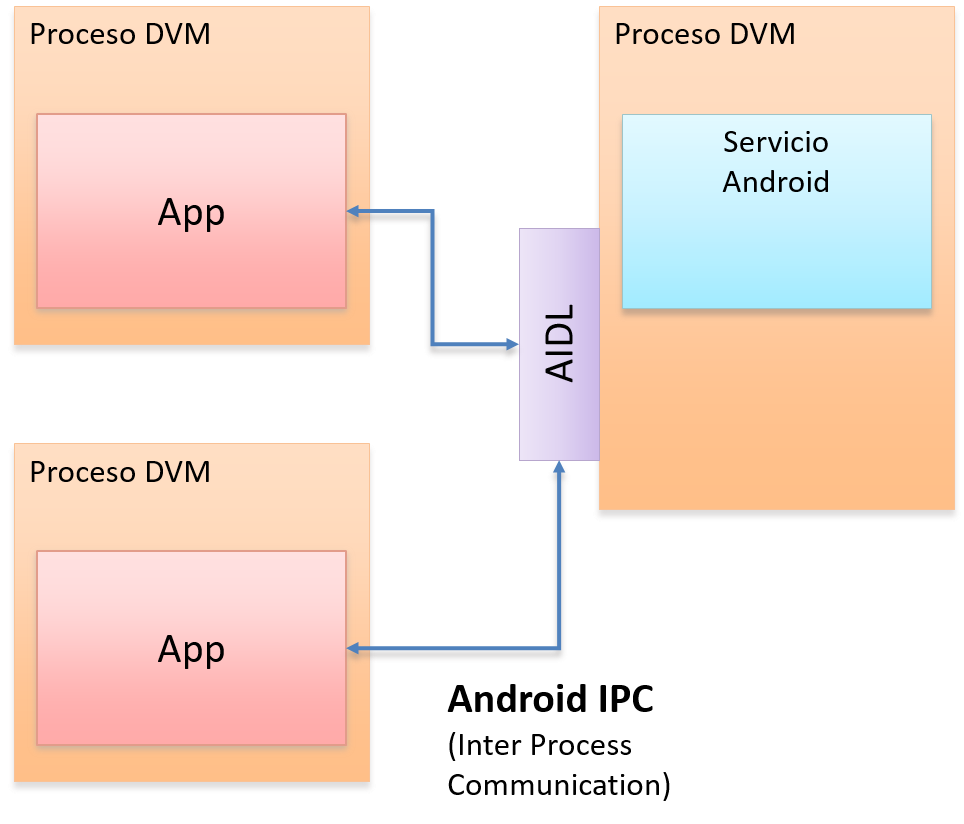
\includegraphics[width=1\columnwidth]{../capitulo-5/graphics/hardroid_func}
\par\end{center}

\end{columns}

\end{frame}
%
\begin{frame}{HAR en Android}

\framesubtitle{HARDroid: M�dulos Funcionales}

\setbeamercovered{transparent}
\begin{columns}[t]

\column{0.30\textwidth}
\begin{itemize}[<+->]
\item Integraci�n \structure{AIDL} 
\item Manejo de Sesi�n
\item Procesamiento de muestras
\item Reconocimiento de Actividades
\item Captura de se�ales
\end{itemize}

\column{0.70\textwidth}
\begin{center}
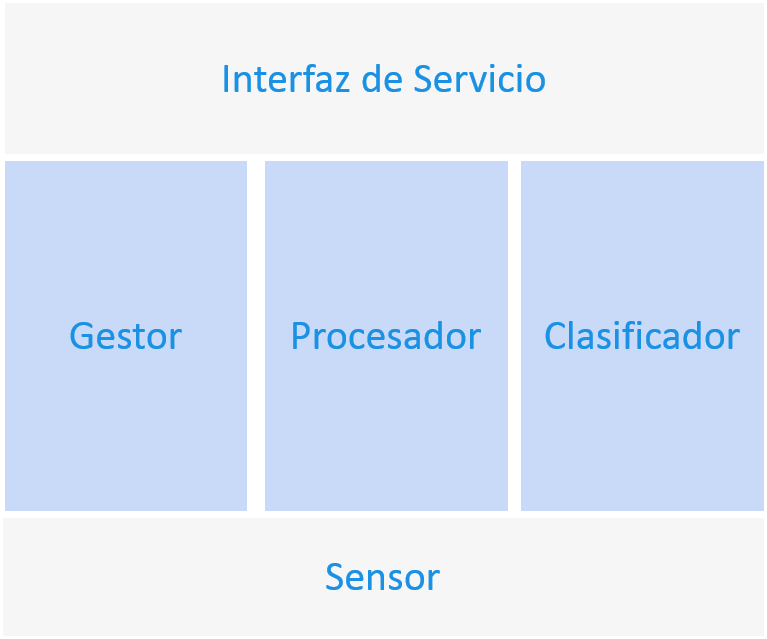
\includegraphics[width=0.9\columnwidth]{propuesta/graphics/hardroid}
\par\end{center}

\end{columns}

\end{frame}
%
\begin{frame}{HAR en Android}

\framesubtitle{HARDroid: Mecanismo de Integraci�n}
\begin{center}
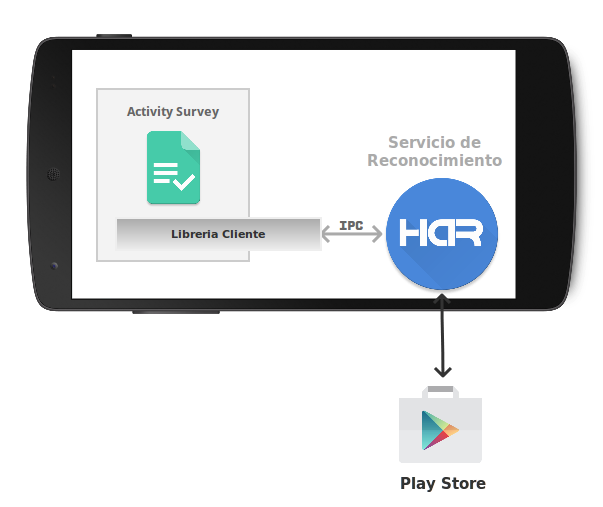
\includegraphics[width=0.5\columnwidth]{propuesta/graphics/archi_ipc}
\par\end{center}
\begin{block}{Nota}
Servicio y Aplicaci�n disponibles en \structure{Google Play Store}
\end{block}
\end{frame}
%
\begin{frame}{HAR en Android}

\framesubtitle{Activity Survey: M�dulos Funcionales}

\setbeamercovered{transparent}
\begin{columns}[t]

\column{0.30\textwidth}
\begin{itemize}[<+->]
\item Presentaci�n
\item Identificaci�n
\item Encuesta guiada
\item Preferencias de comunicaci�n y notificaci�n
\item Almacenamiento y sincronizaci�n
\end{itemize}

\column{0.70\textwidth}
\begin{center}
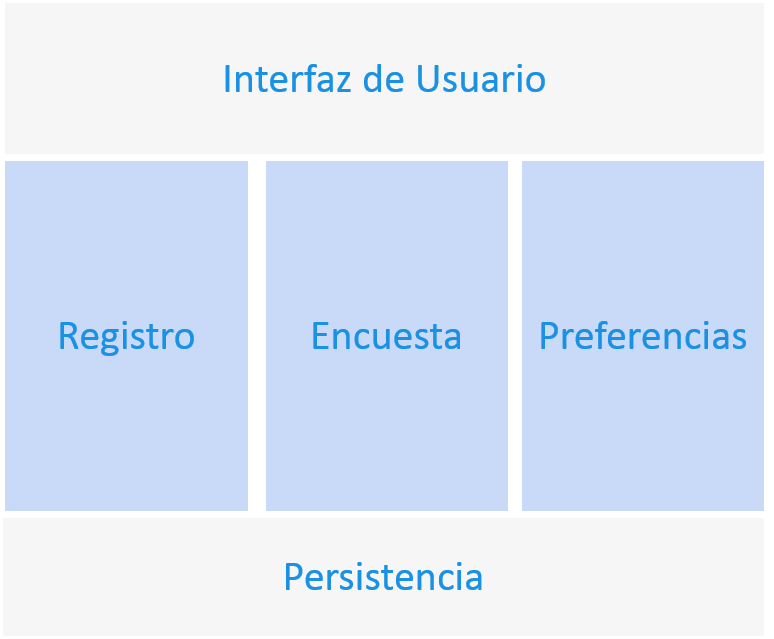
\includegraphics[width=0.9\columnwidth]{propuesta/graphics/activity_survey}
\par\end{center}

\end{columns}

\end{frame}
%
\begin{frame}{HAR en Android}

\framesubtitle{Activity Survey: Componentes Funcionales}
\begin{center}
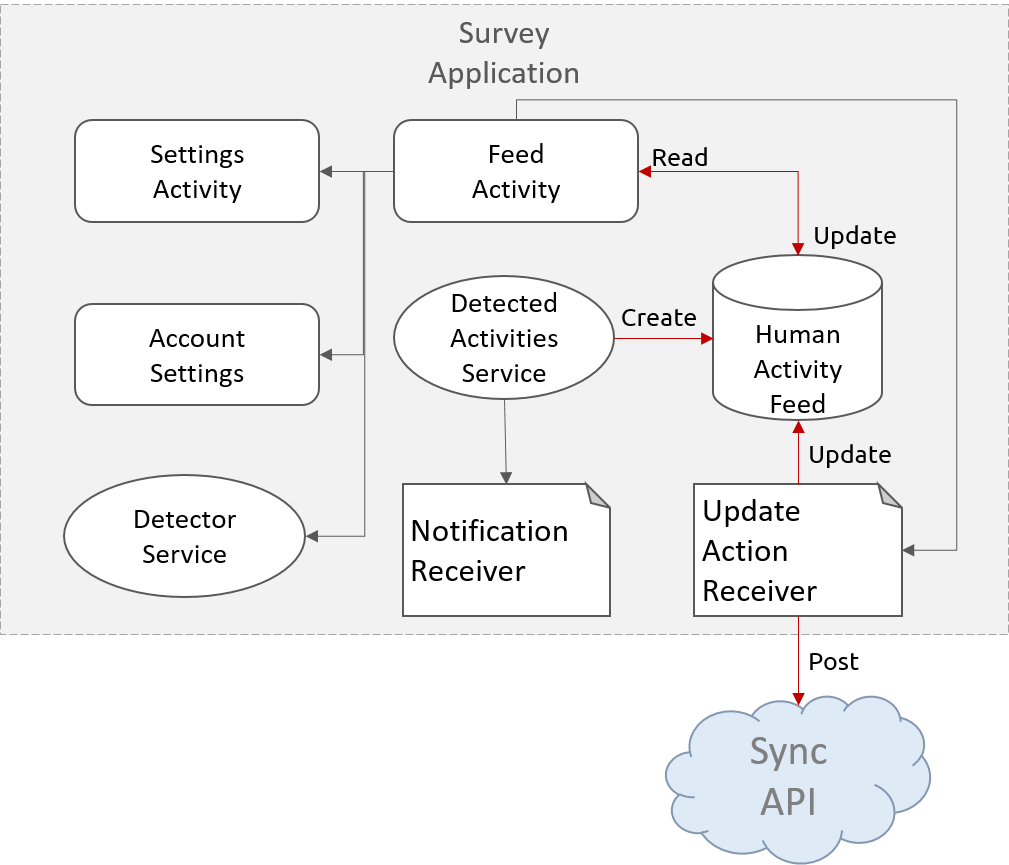
\includegraphics[width=0.65\columnwidth]{../capitulo-5/graphics/act_surv_diag}
\par\end{center}
\end{frame}




\section{Resultados}
\begin{frame}{Resultados}

\framesubtitle{Validaci�n del Clasificador}

\end{frame}
%
\begin{frame}{Resultados}

\framesubtitle{Verificaci�n de la clasificaci�n}

\end{frame}
%
%
\begin{frame}{Resultados}

\framesubtitle{Discusi�n}

\end{frame}
%


\end{document}
